
\section{The pump from the outside}


\todo{include figure with hydraulic circuit}

A very simple hydraulic circuit is illustrated in figure
\ref{fig:hydraulic1}, in which a pump elevates a volumetric flow rate
$\vFlow$ of a liquid from reservoir a to b. The pump therefore needs
needs to increase the pressure and kinetic energy of the liquid of the
liquid to overcome the \emph{hydraulic head} of the circuit 
\begin{align*}
  \dhead_{ab} = \frac{\pres_b - \pres_a}{\dens \grav} + z_b - z_a
\end{align*} as well as the \emph{circuit head loss} $\loss_{ab} =
\loss_{ai} + \loss_{ob}$ generated by the friction in the piping
before and aft of the pump, with $i$ and $o$ adequately chosen
measurement stations near the in- and outlet of the pump.

\subsection{Pump total dynamic head}

We now characterize the action of the pump by the increase $\head_p$
of the total hydrodynamic head it provides as a function of the
volumetric flow rate $\vFlow_p$. The pump \emph{total dynamic head} is
the head increase provided by the pump, measured between the in- and
outlet measurement stations:
\begin{align*}
  \dhead_p = \frac{\pres_o - \pres_i}{\dens \grav} +
  \frac{\vel_o^2 - \vel_i^2}{2\grav} + z_o - z_i
\end{align*}
The measurement of the pump total dynamic head proceeds using static
head measurements. For convenience, the static head is specified with
respect to the inlet $i$ and atmospheric pressure. The measurement
stations $i$ and $o$ should not be too close to the pump such that
fully developed conditions are found in the pipe, but not too far
either since otherwise friction losses in the piping may modify the
measurements. When in- and outlet diameters $D_i$ resp. $D_o$ are
equivalent, the velocity (distribution) in the pipe, and the
corresponding dynamic head, will be the same, such that the pump total
head can be directly deduced from the difference in manometric head at
in- and outlet:
\begin{align*}
  \dhead_p = \frac{\pres_o - \pres_i}{\dens \grav} + z_o - z_i
\end{align*}
In the other case, we need to add the change in dynamic head; the
latter is estimated using the \emph{bulk velocity} $\bar \vel$, computed
from the volumetric flow rate and the pipe diameters to find
\begin{align*}
  \dhead_p 
  &\approx 
  \frac{\pres_o - \pres_i}{\dens \grav} +
  \frac{\bar \vel_o^2 - \bar \vel_{i}^2}{2\grav} + 
  z_o - z_i \\
  &= 
  \frac{\pres_o - \pres_i}{\dens \grav} + 
  \frac{8 Q^2}{\pi}~\frac{D_i^2 - D_o^2}{2 \grav D_i^2 D_o^2} + 
  z_o - z_i
\end{align*}

Conservation of mechanical energy allows us to relate the difference
in manometric head between the reservoirs upstream (a)
resp. downstream (a) of the pump to that at the corresponding
measurement stations. Since the fluid in the reservoirs is at rest, we
have $\vel_a \approx 0$ and $\vel_b \approx 0$, and therefore
\begin{align*}
  \frac{\pres_a}{\dens \grav} + z_a 
  &= \frac{\pres_i}{\dens \grav} + 
  \frac{\vel_i^2}{2 \grav} + z_i + \loss_{ai} \\
  \frac{\pres_b}{\dens \grav} + z_b 
  &= \frac{\pres_o}{\dens \grav} +
  \frac{\vel_o^2}{2 \grav} + z_o - \loss_{ob}
\end{align*}
Therefore we find
\begin{align*}
  \dhead_p = 
  \underbrace{\frac{\pres_b - \pres_a}{\dens \grav} + z_b - z_a}_{\head_{ab}} + 
  \underbrace{\loss_{ai} + \loss_{ob}}_{\loss_{ab}}
\end{align*}
where we lump the circuit losses in $\loss_{ab}$. The hydraulic head
diagram of the circuit is then shown in figure
\ref{fig:headDiagramCircuit}.
\begin{figure}[!h]
  \centering{\tikzsetnextfilename{headDiagramCircuit}
\begin{tikzpicture}

  \scriptsize
  
  \def\vU{6}
  
  \def\hA{25} %% reference manometric head (upstream reservoir)
  \def\lAS{0.5*\vU}         %% losses A -> sump
  \def\hS{\hA-\lAS}
  \def\lSI{2*\vU}         %% losses sump -> inlet
  \def\hI{\hS-\lSI}

  \def\hp{80}         %% total dynamic head of the pump
  
  \def\hO{\hI+\hp}
  
  \def\vD{6}
  \def\lOD{2*\vD}
  \def\hD{\hO-\lOD}
  \def\hB{\hD-\vD}
  
  \begin{axis}[
    width = \textwidth,
    height =0.4\textheight,
    xtick = data,
    xticklabels = {Reservoir a,Sump,Pump,Discharge,Reservoir b},
    ytick = \empty,
    axis lines = center,
    xmin = 0,
    xmax = 5,
    ymin = 0,
    ymax = 100,
    % xlabel = $station$,
    % ylabel = $\head$,
    legend style   = {draw=none,anchor=west,at={(0.1,0.5)}},
    legend entries = {total head,static head}
    ],
    \addplot [black,line width=1.5pt] coordinates {
      (0.5,\hA) 
      (1.5,\hS) 
      (2.5,\hI) 
      (2.5,\hO) 
      (3.5,\hD) 
      (4.5,\hD-\vD)};
    \addplot [dashed,line width=1.5pt] coordinates {
      (0.5,\hA) 
      (1.5,\hS-\vU) 
      (2.5,\hI-\vU) 
      (2.5,\hO-\vD) 
      (3.5,\hD-\vD) 
      (4.5,\hB)};
    
    \addplot [dashed] coordinates {(0.5,0) (0.5,\hA)};
    \addplot [dashed] coordinates {(1.5,0) (1.5,\hS)};
    \addplot [dashed] coordinates {(2.5,0) (2.5,\hI)};
    \addplot [dashed] coordinates {(2.5,0) (2.5,\hO)};
    \addplot [dashed] coordinates {(3.5,0) (3.5,\hD)};
    \addplot [dashed] coordinates {(4.5,0) (4.5,\hB)};
    
    \addplot [dashed] coordinates {(0,\hA) (4.6,\hA)}
    node [pos=0.05,left,above]{$\head_a$};
    \addplot [dashed] coordinates {(0,\hB) (4.6,\hB)}
    node [pos=0.05,left,above]{$\head_b$};
    
    \addplot [dashed] coordinates {(2.4,\hI) (3,\hI)};
    \addplot [dashed] coordinates {(2.4,\hO) (4.6,\hO)};
    \addplot [<->,>=latex] 
    coordinates {(2.9,\hI) (2.9,\hO)} 
    node [midway,right] {$\dhead_p$};
    \addplot [<->,>=latex] 
    coordinates {(4.5,\hB) (4.5,\hO)} 
    node [midway,left] {$\loss_{ob}$};
    \addplot [<->,>=latex] 
    coordinates {(2.5,\hA) (2.5,\hI)} 
    node [midway,left] {$\loss_{ai}$};
    
  \end{axis}

\end{tikzpicture}}
  \caption{Hydraulic head diagram for the circuit}
  \label{fig:headDiagramCircuit}
\end{figure}

\subsection{Power and efficiency}

The total head provides us with a measure of the useful energy
conveyed to the fluid \emph{per unit of weight}. The corresponding
\emph{total hydraulic power} $\power_p$ developed by the pump is then
given by
\begin{align*}
  \power_p = \mFlow \frac{\Delta p_t}{\dens} = \dens \grav \vFlow_p \dhead_p 
\end{align*}
The pump absorbs an electric power $\power_e$; the latter is only
partially converted into hydraulic power, since it also compensates
for the mechanical losses, \eg occuring in the bearings of the shaft,
as well as all of the hydraulic losses in the pump. We then define the
\emph{global efficiency} of the pump as
\begin{align*}
  \eff_p = 
  \frac{\power_p}{\power_e}
\end{align*}
We will come back to the nature and origins of the mechanical and
hydraulic losses in the next section. Turning back to the circuit, the
useful work is determined by the circuit head $\dhead_{ab}$, whereas
the pump needs to provide a higher head $\dhead_p$ since it also
compensates for the circuit losses $\loss_{ab}$. Therefore, we can
define the hydraulic efficiency of the circuit as
\begin{align*}
  \eff_{ab} = \frac{\dhead_{ab}}{\dhead_p} = 
  \frac{\dens \grav \vFlow_p \dhead_{ab}}{\dens \grav \vFlow_p \dhead_p} =
  \frac{\power_{ab}}{\power_p}
\end{align*}
Therefore, the efficiency of the installation is given by
\begin{align*}
  \eff = \eff_{ab} ~\eff_p = \frac{\power_{ab}}{\power_e} 
\end{align*}

\subsection{Characteristic curves}

The user of a pump is interested in the following operating parameters
\begin{itemize}
\item hydraulic parameters, including flow rate $\vFlow_p$, and total
  dynamic $\dhead_p$ or manometric head $\dhead_m$;
\item mechanical parameters, including power consumption $\power_e$
  and rotational speed $\rot$.
\end{itemize}
as any other important parameter can be easily deduced:
\begin{itemize}
\item the torque on the shaft $\torque_e = \power_e / \rot$;
\item the total hydraulic power $\power_p = \dens \grav \vFlow_p \dhead_p$;
\item the total efficiency $\eff_e=\power_p/\power_e$
\end{itemize}
The pump is then characterized by two relations between the
fundamental parameters
\begin{align*}
  \dhead_p &= \dhead_p(\vFlow_p,\rot)  \\
  \power_e &= \power_e(\vFlow_p,\rot) 
\end{align*}
which are called the \emph{characteristic surfaces}. At constant
rotational speed speed, these reduce to the \emph{characteristic
  curves}
\begin{align*}
  \dhead_p &= \dhead_p(\vFlow_p)  \\
  \power_e &= \power_e(\vFlow_p) 
\end{align*}
These curves are typically obtained experimentally. The theoretical
prediction results from combining the Euler equation of turbomachinery
with different models for loss, imperfect guidance etc.

\todo{include measured curves and references for prediction}
\todo{Determine working point by intersection}
\todo{Parallel and serial operation}


%%% Local Variables: 
%%% mode: latex
%%% TeX-master: "../MECA0467"
%%% End: 
